% Estas slides tienen que abrirse con el programa pdfpc que soporta videos embebidos
% el comando es: pdfpc -g slides.pdf
% para los videos se requiere ubuntu-restricted-extras
% para la bibliografía se requiere biber y configurar texstudio

%\documentclass[compress,handout]{beamer}
\documentclass[aspectratio=169,compress]{beamer}

% add beamer preamble
% In this preamble should go only package and settings related with beamer

% Theme customization
\setbeamertemplate{itemize item}[rectangle] % configure itemize
\setbeamertemplate{itemize subitem}[circle] % configure itemize
\setbeamertemplate{itemize subsubitem}[triangle] % configure itemize
\setbeamertemplate{navigation symbols}{} % remover simbolos de navegacion de las slides
\usefonttheme[onlymath]{serif} % simbolos matematicos en serif (Como es en latex original)
\setbeamersize{text margin left=3mm,text margin right=3mm} 

\setbeamertemplate{blocks}[rounded] % blocks corners rounded
\setbeamercolor{block body}{bg=blue!12,fg=black} % color of blocks
\setbeamertemplate{caption}{\raggedright\insertcaption\par} % elimina la palabra "Figura" del caption

\usepackage[overridenote]{pdfpc} % requires to download manually pdfpc.sty package from https://www.ctan.org/pkg/pdfpc
% para instalar el pdfpc.sty seguir las instrucciones en https://micropore.wordpress.com/2009/11/28/texhash/

%\setbeameroption{show notes on second screen=right} % visualize slides with notes using beamerpresenter slides.pdf

% HOW TO SHOW ADDITIONAL SLIDES%
\newif\ifadditional % conditional to show additional slides
%\additionaltrue   % uncomment to show additional slides
\additionalfalse % uncomment to show without additional slides

% Reference cite without footnote mark
\newrobustcmd*{\footfullcitenomark}{%
    \AtNextCite{%
        \let\thefootnote\relax
        \let\mkbibfootnote\mkbibfootnotetext}%
    \footfullcite}


% add latex preamble
% para la bibliografía se requiere biber y configurar texstudio

% Latex packages
\usepackage[utf8]{inputenc}
\usepackage[T1]{fontenc} % para copiar acentos en español del pdf y permite acentos en las notas
\usepackage[english]{babel}
\usepackage[per-mode = symbol]{siunitx} % para manejar las unidades
\usepackage{multimedia} % to add videos with \movie command
\usepackage{multirow}
\usepackage{graphicx}
\usepackage{xcolor}
\usepackage{amsmath} % bmatrix
\usepackage[makeroom]{cancel} % \cancel to cancel terms in math equations
\renewcommand{\CancelColor}{\color{red}} % set red color for \cancel command
\usepackage[caption=false]{subfig} % caption = false elimina la palabra "Figura" del caption
\usepackage{import} % para el comando import (se usa para pdf_tex)
\captionsetup[subfigure]{labelformat=empty} % remover el indice del caption de la subfigura
\usepackage{booktabs} % \toprule \midrule \bottomrule
\usepackage[backend=biber]{biblatex} % set biber to format references. Must configure Biber in Texstudio
\usepackage{csquotes} % to remove warning triggered by biblatex and babel
\usepackage{algorithm} % to put captions to the algorithmics environmets
\usepackage{algpseudocode} % to write algorithm
\usepackage{tikz} % to use tikz
\usepackage[export]{adjustbox} %valign in subfloat
\usepackage{colortbl} % to paint cells in a table

% Color commands for annotations
\newcommand\TODO[1]{\textbf{\textcolor{red}{#1}}} %  TODO notes

% Graphic paths
\graphicspath{{./images/}}

% listings configuration for C code
\usepackage{listings} % code
\definecolor{commentgreen}{RGB}{2,112,10}
\definecolor{eminence}{RGB}{108,48,130}
\definecolor{weborange}{RGB}{255,165,0}
\definecolor{frenchplum}{RGB}{129,20,83}

\lstset{ % spanish characters for listings package
	inputencoding=latin1,
    columns=fullflexible,
	breaklines=true,
	tabsize=2,
	showstringspaces=false,
	basicstyle=\ttfamily,
	backgroundcolor=\color{lightgray}, % Choose background color
	literate={á}{{\'a}}1
	{ã}{{\~a}}1
	{é}{{\'e}}1
	{ó}{{\'o}}1
	{í}{{\'i}}1
	{ñ}{{\~n}}1
	{¡}{{!`}}1
	{¿}{{?`}}1
	{ú}{{\'u}}1
	{Í}{{\'I}}1
	{Ó}{{\'O}}1
    {-}{-}1
}

\lstdefinestyle{cpp}{ % spanish characters for listings package
    language=C++,
   	commentstyle=\color{commentgreen},
    keywordstyle=\color{eminence},
    stringstyle=\color{red},
    emph={int,char,double,float,unsigned,void,bool},
    emphstyle={\color{blue}}
}

\lstdefinestyle{bash}{ % spanish characters for listings package
	language=Bash
}

\lstdefinestyle{xml}{
	language=XML,
	morekeywords={encoding,xs:schema,xs:element,xs:complexType,xs:sequence,xs:attribute}
}

\lstdefinestyle{cmake}{
	language=make, % there is no cmake support in listings
}

\lstdefinestyle{python}{
    language=python,
}


%%%%% PARA QUE EN LAS TABLAS SE PUEDA PONER UN SALTO DE LINEA DENTRO DE UNA CELDA
\newcommand{\specialcell}[2][c]{%
    \begin{tiny}
        \begin{tabular}[#1]{@{}c@{}}#2\end{tabular}  
    \end{tiny}
}
%%%%%%%%%%%%%%%%%%%%%%%%%%%%%%%%%%%%%%%%%%%%%%%%%%%%%%%%%%%%%%%%%%%%%%%%

%%%%% PARA QUE LAS TABLAS TENGAN TODAS LAS COLUMNAS CENTRADAS Y DE IGUAL TAMAÑO
\usepackage{tabularx}
\renewcommand{\tabularxcolumn}[1]{>{\centering\arraybackslash}m{#1}}
%%%%%%%%%%%%%%%%%%%%%%%%%%%%%%%%%%%%%%%%%%%%%%%%%%%%%%%%%%%%%%%%%%%%%%%%



% add math preamble
\usepackage{amsmath}
\usepackage{amssymb}
\usepackage{amsopn}
\usepackage{mathtools}

% set matrix maximum length
\setcounter{MaxMatrixCols}{20}

% math
\renewcommand{\vec}[1]{\boldsymbol{\mathbf{#1}}}
\newcommand{\norm}[1]{\lVert#1\rVert}

% Declare arg max and arg min functionss
\DeclareMathOperator*{\argmax}{arg\,max}
\DeclareMathOperator*{\argmin}{arg\,min}

% Declare atan2 
\DeclareMathOperator{\atantwo}{atan2}

% Homogeneous decoration function
\newcommand{\homo}[1]{\dot{#1}}


% Declare projection as math function
\DeclareMathOperator{\proj}{proj}
\newcommand{\fromCoord}[2]{{#1}_\mathrm{#2}}
\newcommand{\toCoord}[2]{\prescript{\mathrm{#2}}{}{#1}}
\newcommand{\worldCoordSystem}{\mathrm{W}}
\newcommand{\bodyCoordSystem}{\mathrm{B}}
\newcommand{\cameraCoordSystem}{\mathrm{C}}
\newcommand{\origin}{\vec{o}}
\newcommand{\point}{\vec{p}}
\newcommand{\worldPoint}{\toCoord{\point}{\worldCoordSystem}}
\newcommand{\imagePoint}{\vec{u}}
\newcommand{\cameraPoint}{\toCoord{\point}{\cameraCoordSystem}}
\newcommand{\homoWorldPoint}{\toCoord{\homo{\point}}{\worldCoordSystem}}
\newcommand{\homoImagePoint}{\homo{\imagePoint}}
\newcommand{\homoCameraPoint}{\toCoord{\homo{\point}}{\cameraCoordSystem}}
\newcommand{\measurement}{\vec{z}}
\newcommand{\prediction}{\hat{\vec{z}}}
\newcommand{\seMatrix}{\vec{\xi}}
\newcommand{\transform}[2]{\toCoord{\fromCoord{\seMatrix}{#2}}{#1}}
\newcommand{\pointCoord}[1]{\toCoord{\point}{#1}}
\newcommand{\rotation}{\vec{R}}
\newcommand{\rotationCoord}[2]{\toCoord{\fromCoord{\rotation}{#2}}{#1}}
\newcommand{\translation}{\vec{t}}
\newcommand{\translationCoord}[2]{\toCoord{\fromCoord{\translation}{#2}}{#1}}
\newcommand{\intrinsicMatrix}{\vec{K}}
\newcommand{\principalPoint}{\vec{c}}
\newcommand{\reprojectionError}{u}
\newcommand{\projectionMatrix}{\vec{P}}
\newcommand{\cameraCenter}{\vec{o}}
\newcommand{\worldCameraCenter}{\toCoord{\cameraCenter}{\worldCoordSystem}}
\newcommand{\essentialMatrix}{\vec{E}}
\newcommand{\fundamentalMatrix}{\vec{F}}
\newcommand{\inverse}[1]{{#1}^{-1}}
\newcommand{\epipole}{\vec{e}}

% Localization (State Estimation)
\newcommand{\state}{x}
\newcommand{\observation}{z}
\newcommand{\controlCommand}{u}
\newcommand{\covariance}{\Sigma}
\newcommand{\motionModelNoise}{\epsilon}
\newcommand{\measurementModelNoise}{\delta}
\newcommand{\motionModelFunction}[1]{g\left( #1 \right)}
\newcommand{\observationModelFunction}[1]{h\left( #1 \right)}
\newcommand{\motionParametersCovariance}{R}
\newcommand{\observationModelCovariance}{Q}
\newcommand{\motionModelJacobian}{G}
\newcommand{\observationModelJacobian}{H}
\newcommand{\kalmanGain}{K}
\newcommand{\normalDistribution}[2]{\mathcal{N}\left( {#1}, {#2} \right)}
\newcommand{\motionModelJacobianControl}{V}
\newcommand{\motionModelCovariance}{M}
\newcommand{\stateEvolutionMatrix}{A}

% Mapping slides
\newcommand{\map}{m}
\newcommand{\mapRandomVariable}{m}

% SLAM slides
\newcommand{\informationMatrix}{\vec{\Omega}}
\newcommand{\error}{\vec{e}}
\newcommand{\observationBold}{\vec{z}}
\newcommand{\stateBold}{\vec{x}}
\newcommand{\jacobian}{\vec{J}}
\newcommand{\linearSystemb}{\vec{b}}
\newcommand{\linearSystemH}{\vec{H}}


% Motion Planning slides
\newcommand{\workSpace}{\mathcal{W}}
\newcommand{\obstaclesSet}{\mathcal{O}}
\newcommand{\robotInConfiguration}{\mathcal{A}}
\newcommand{\robotConfiguration}{q}
\newcommand{\configurationSpace}{\mathcal{C}}
\newcommand{\freeConfigurationSpace}{\configurationSpace_{free}}
\newcommand{\obstableConfigurationSpace}{\configurationSpace_{obs}}
\newcommand{\goalSet}{\configurationSpace_{goal}}
\newcommand{\startConfiguration}{\robotConfiguration_{I}}
\newcommand{\goalConfiguration}{\robotConfiguration_{G}}
\newcommand{\continuousPath}{\tau}
\newcommand{\motionLaw}{\gamma}
\newcommand{\robotActionSpace}{\mathcal{U}}


% Motion model
\newcommand{\position}{\vec{p}}
\newcommand{\orientation}{\vec{O}}
\newcommand{\orientationQuaternion}{\vec{q}}
\newcommand{\predictedPosition}{\hat{\vec{p}}}
\newcommand{\predictedOrientationQuaternion}{\hat{\vec{q}}}
\newcommand{\linearVelocity}{\vec{v}}
\newcommand{\angularVelocity}{\vec{\omega}}

\DeclareMathOperator{\slerpOp}{slerp}
\newcommand{\slerp}[1]{\slerpOp{\left( #1 \right)}}

% Map structure
\newcommand{\keyframesSet}{K}
\newcommand{\mapPointsSet}{P}
\newcommand{\observedMapPoints}{O}
\newcommand{\covisibilityKeyframes}{CK}
\newcommand{\localMap}{local\_map}

% Bundle Adjutment
\newcommand{\update}{\vec{\delta}}
\newcommand{\incremental}{\hat{\update}}


% Loop Closure names

% scaled operators and letters to fancy view
\newcommand{\sminus}{\scalebox{0.5}[1.0]{$-$}}
\newcommand{\splus}{\scalebox{0.6}[0.6]{$+$}}
\newcommand{\curr}{c}
\newcommand{\sind}[1]{\scalebox{0.6}[0.6]{$#1$}}
\newcommand{\ind}[1]{\scalebox{0.7}[0.7]{$#1$}}

\newcommand{\keyframe}{\vec{K}}
\newcommand{\bowVector}{\vec{v}}
\newcommand{\lcError}{\vec{\Omega}}
\newcommand{\relativeTransformation}{\seMatrix}
\DeclareMathOperator{\interpolate}{interpolate}

\newcommand{\relativeMotion}{\vec{\delta}}
\newcommand{\groundTruth}[1]{{#1}^{*}}

% definición del operador rot()
\DeclareMathOperator{\rotationOp}{rot}
\newcommand{\getRotation}[1]{\rotationOp{\left( #1 \right)}}

\DeclareMathOperator{\translationOp}{trans}
\newcommand{\getTranslation}[1]{\translationOp{\left( #1 \right)}}









% add bibliography resource
\renewcommand*{\bibfont}{\footnotesize} % change bibliograhy size
\bibliography{../../common/bibliography.bib}

\subtitle{Mapping}
\title{Mobile Robotics}
\author{Taihú Pire}
\institute{Robotics Laboratory}
\titlegraphic{
\includegraphics[width=0.4\textwidth]{images/cifasis_logo.pdf}}
\date{}


\begin{document}

	% add title page
	\frame{\titlepage}

	\section{Map: Occupancy Grid}
	\begin{frame}
    \frametitle{Occupancy Grid Maps}
    \note{information taken from https://youtu.be/v-Rm9TUG9LA}
    
    \begin{itemize}
    \item Representation of the environment generally used by mobile robots.
    \item These types of maps store information about which areas of the map are occupied (there are obstacles) and which are free (can be navigated). They can be thought of as a "site plan."
    \item They allow for path planning.
    \end{itemize}
    
    \end{frame}
    
    \begin{frame}
    \frametitle{Motivation: Why Map}
    \note{information taken from https://youtu.be/v-Rm9TUG9LA}
    
    \begin{itemize}
    \item Maps are required for most robotics tasks such as localization, planning, etc.
    \item Tasks that require an understanding of the environment (semantic information)
    \item Learning maps from sensor measurements is one of the fundamental tasks of mobile robotics.
    \end{itemize}
\end{frame}

\begin{frame}
    \frametitle{Sensors for Mapping}
    \note{Information taken from https://youtu.be/v-Rm9TUG9LA}
    
    \note{Exteroceptive sensors that allow us to measure the environment}
    
    \begin{figure}[!h]
    \centering
    \subfloat[\scriptsize Camera]
    {
    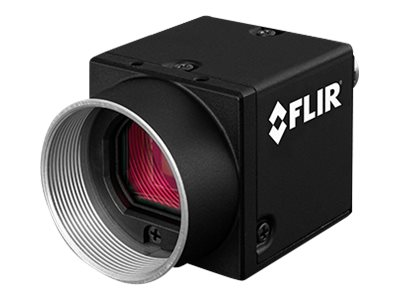
\includegraphics[width=0.15\columnwidth,valign=m]{./images/flir_blackfly_s_camera.jpg}
    }
    \subfloat[\scriptsize Stereo Camera]
    {
    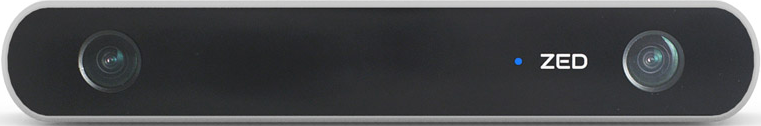
\includegraphics[width=0.2\columnwidth,valign=m]{./images/stereo_camera_zed.png}
    }
    \subfloat[\scriptsize Camera \SI{360}{\degree}]
    { 
    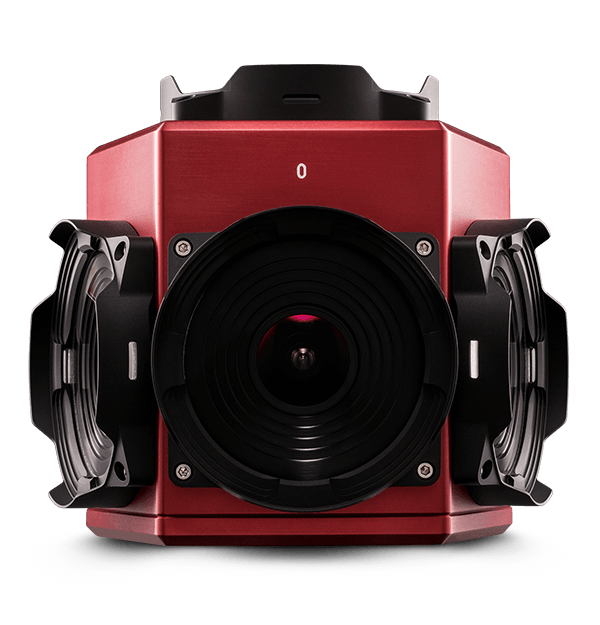
\includegraphics[width=0.1\columnwidth,valign=m]{./images/ladybug5plus_360_camera.png}
     }
     \subfloat[\centering \scriptsize Structured Light Chamber]
     {
     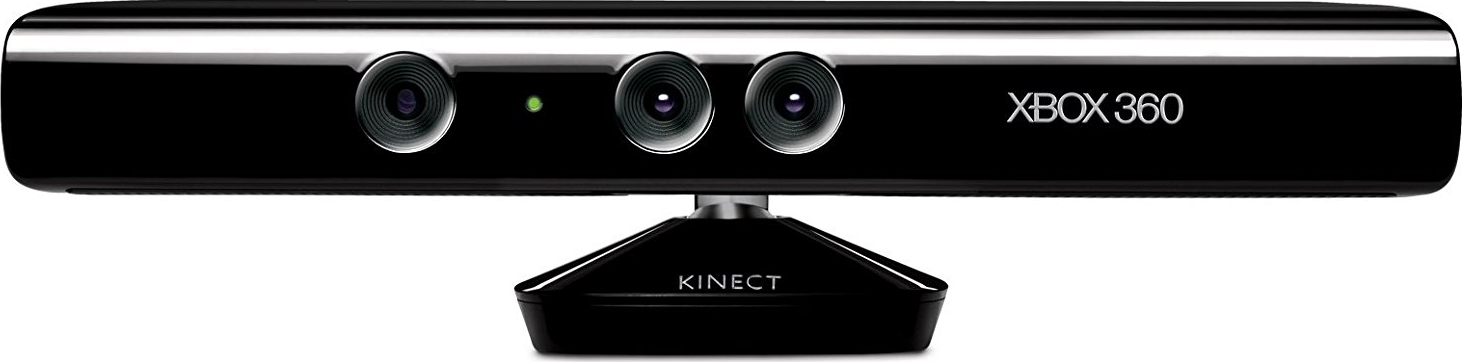
\includegraphics[width=0.2\columnwidth,valign=m]{./images/structured_light_kinect.png}
     }\\
     \subfloat[\scriptsize ToF Camera]
     {
     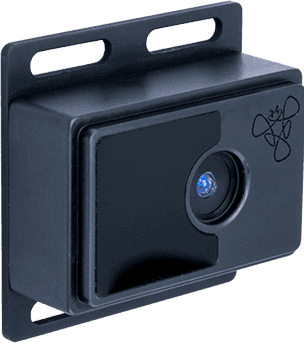
\includegraphics[width=0.15\columnwidth,valign=m]{./images/terabee_time_of_flight_camera.png}
     }
     \subfloat[\scriptsize Event Camera]
     {
     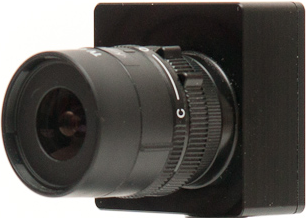
\includegraphics[width=0.2\columnwidth,valign=m]{./images/event_camera_dvs128.png}
     }
     \subfloat[\scriptsize LiDAR 2D]
     {
     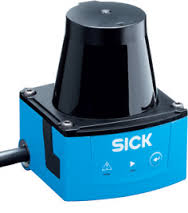
\includegraphics[width=0.15\columnwidth,valign=m]{./images/lidar_sick.jpg}
     }
     \subfloat[\scriptsize LiDAR 3D]
     {
     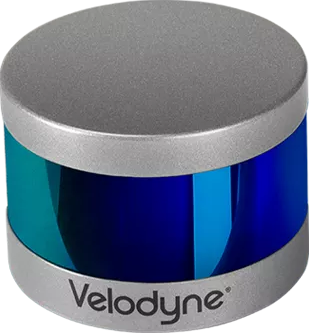
\includegraphics[width=0.15\columnwidth,valign=m]{./images/velodyne_puck.png}
     }
     \end{figure}
    
\end{frame}

\begin{frame}
    \frametitle{Volumetric Maps vs. Features}
    \note{Information taken from https://youtu.be/v-Rm9TUG9LA}
    
    \note{Feature maps store distinctive points of the environment}
    
    \note{The feature map corresponds to a project by Eduardo Nebot in Victoria Park. The yellow dots are the tree trunks.}
    
    \note{Feature maps are only useful for localization, not for navigating the environment, since it is unknown what exists between the points.}
    
    \note{2D volumetric maps can be viewed as a floor plan of a room.}
    
    \note{Volumetric maps explicitly represent the free areas of the environment.}
    
    \begin{figure}[!h]
    \centering
    \subfloat[2D Volumetric Map (Grid map)]
    {
    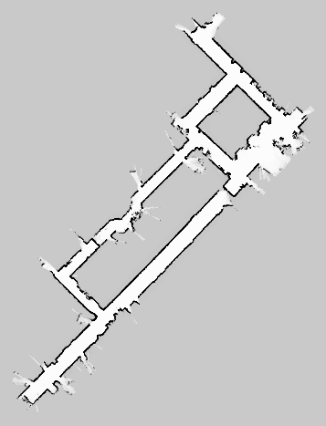
\includegraphics[width=0.23\columnwidth]{./images/volumetric_map_2d.png}
    }
    \subfloat[3D Volumetric Map (Voxel map)]
    {
    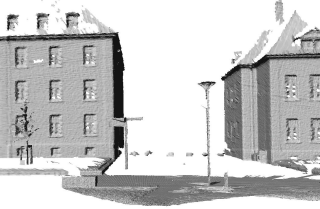
\includegraphics[width=0.3\columnwidth]{./images/volumetric_map_3d.png}
    }
    \subfloat[Voxel map] 2D features]
     {
     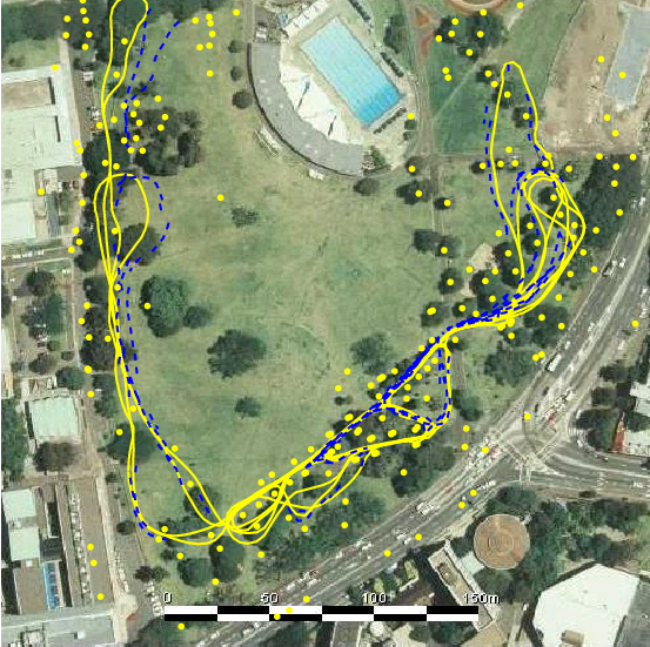
\includegraphics[width=0.3\columnwidth]{./images/feature_map_2d.png}
     }
     \end{figure}
    
\end{frame}

\begin{frame}
    \frametitle{Quadtree}
    \note{información extraída de https://youtu.be/v-Rm9TUG9LA}
    
    
    \begin{figure}
    	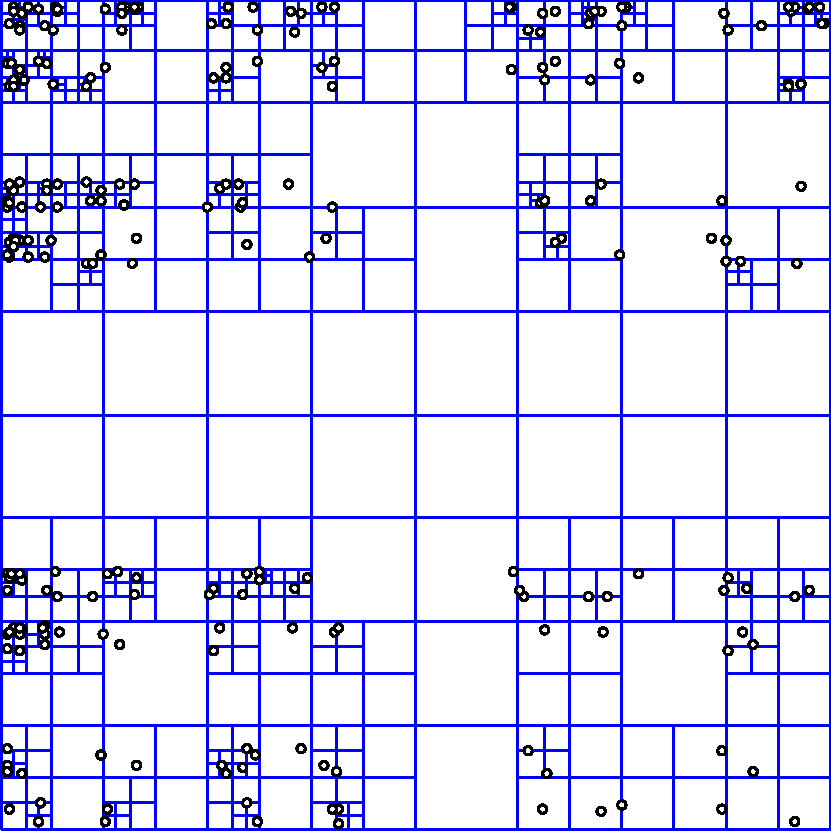
\includegraphics[width=0.5\columnwidth]{./images/quadtree.pdf}
    \end{figure}
    
\end{frame}

\begin{frame}
	\frametitle{Octree (Octomap)}
	\note{información extraída de https://youtu.be/v-Rm9TUG9LA}

	\begin{figure}
		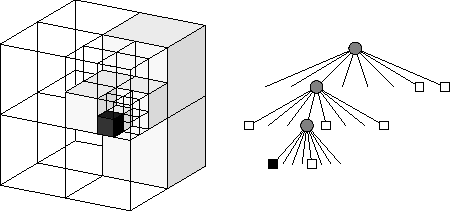
\includegraphics[width=0.5\columnwidth]{./images/octree.pdf}
	\end{figure}
	
	\begin{figure}
		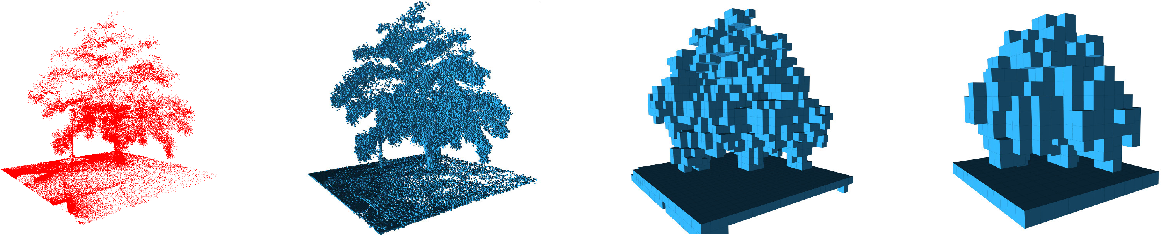
\includegraphics[width=\columnwidth]{./images/octomap.pdf}
	\end{figure}
	
\end{frame}

\begin{frame}
    \frametitle{Mapa de Nube de puntos (Point Cloud Map)}
    \note{información extraída de https://youtu.be/v-Rm9TUG9LA}
    
    
   	\begin{figure}
    	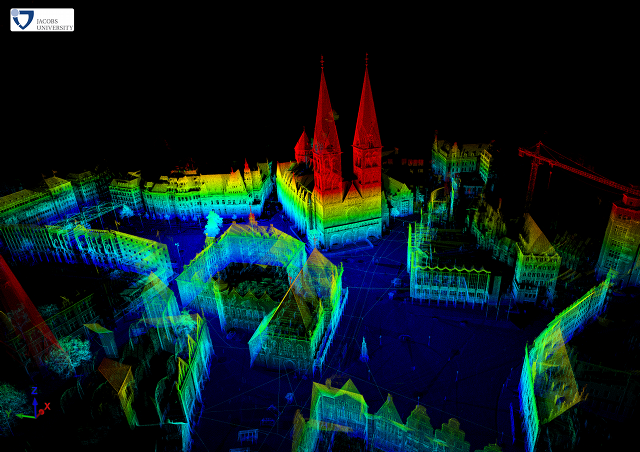
\includegraphics[width=0.6\columnwidth]{./images/point_cloud_map_bremen_city.png}
    \end{figure}
    
\end{frame}

\begin{frame}
    \frametitle{TSDF: Truncated Signed Distance Function}
   
   	\begin{figure}[!h]
	   	\centering
	   	\subfloat[TSDF 2D Function]
	   	{
	   		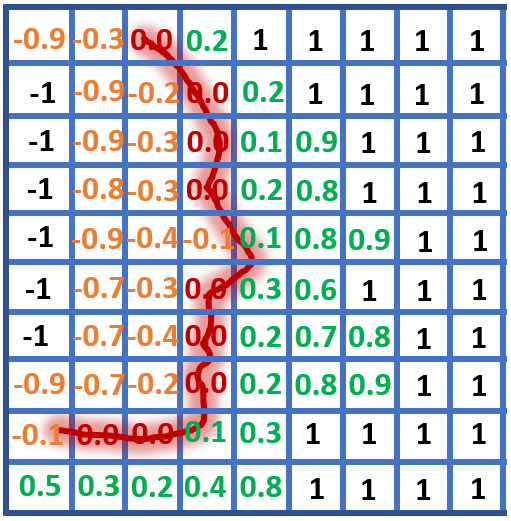
\includegraphics[width=0.45\columnwidth]{./images/tsdf.png}
	   	}
	   	\subfloat[TSDF Reconstruction]
	   	{
	   		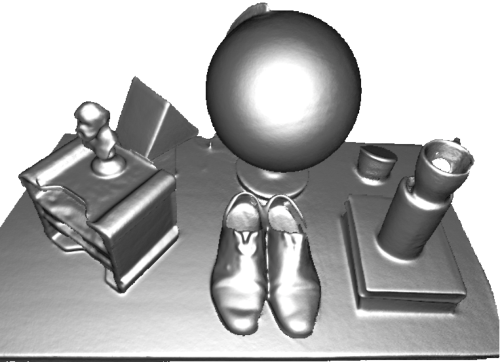
\includegraphics[width=0.45\columnwidth]{./images/tsdf_reconstruction.pdf}
	   	}
   \end{figure}
    
\end{frame}


\begin{frame}
	\frametitle{Mapa Semántico (Semantic Map)}
	\note{información extraída de https://youtu.be/v-Rm9TUG9LA}
	
   	\begin{figure}
    	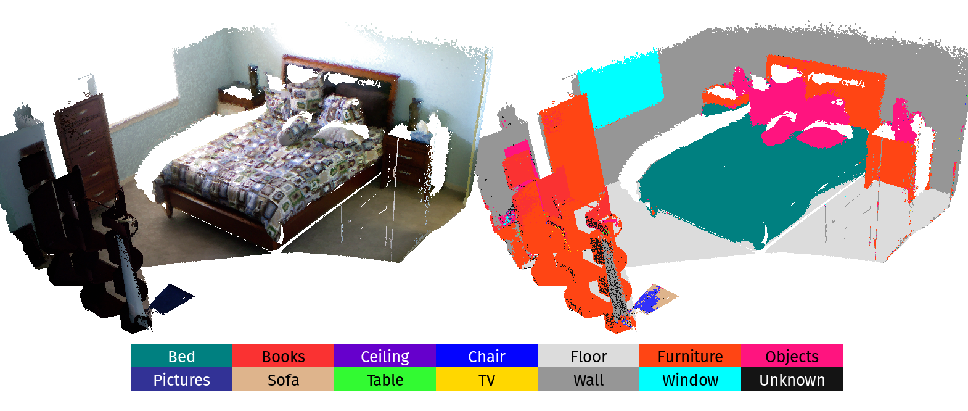
\includegraphics[width=0.8\columnwidth]{./images/semantic_map_semanticfusion.png}
	\end{figure}
	
\end{frame}


\begin{frame}
	\frametitle{Mapa Topológico}
	\note{información extraída de https://youtu.be/v-Rm9TUG9LA}
	
	\begin{figure}
		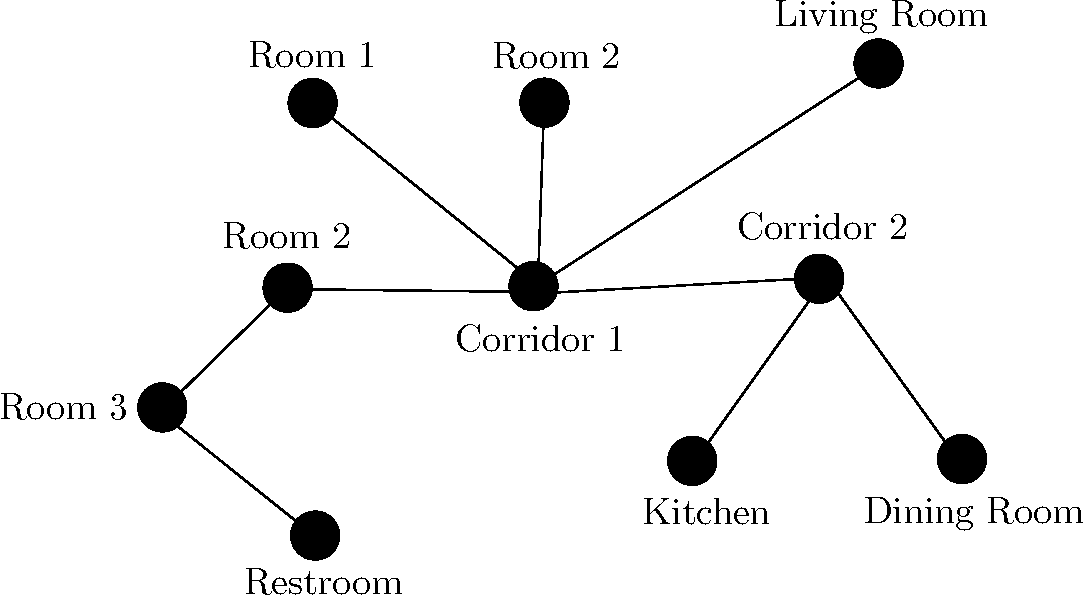
\includegraphics[width=0.8\columnwidth]{./images/topological_map.pdf}
	\end{figure}
	
\end{frame}

\begin{frame}
    \frametitle{Map Reconstruction}
    \note{information taken from https://youtu.be/v-Rm9TUG9LA}
    
    \begin{itemize}
    \item Computing the most likely map given the sensor measurements
    \begin{equation*}
    \map^{*} = \argmax p(\map | \controlCommand_{1}, \observation_{1}, \dots, \controlCommand_{t}, \observation_{t})
    \end{equation*}
    \item However, let's tackle a simpler problem: let's see how to compute the map given the robot's pose (the resolved localization) and the sensor measurements.
    \begin{equation*}
    \map^{*} = \argmax p(\map | \state_{1}, \observation_{1}, \dots, \state_{t}, \observation_{t})
    \end{equation*}
    \end{itemize}
    
    \alert{Solving localization and mapping at the same time is solving the SLAM problem, and we'll see this later.}
    
\end{frame}
    
\begin{frame}
    \frametitle{Grid Maps}
    \note{Information taken from https://youtu.be/v-Rm9TUG9LA}
    
    \note{}
    
    \begin{itemize}
    \item Space Occupancy Map Models
    \item Discretize the world into cells
    \item The grid structure is fixed (the size of the cells and the grid are fixed)
    \item Each cell can be occupied or free
    \item Non-parametric model (i.e., a cell is not parameterized as a Gaussian, for example, but is either free or occupied)
    \item The size of the grid maps can be very memory-intensive (especially in the 3D case)
    \item It does not require a specific feature detector (but rather we use raw sensor measurements)
    \end{itemize}
\end{frame}
    
\begin{frame}
    \frametitle{Occupancy Grid Map Example}
    \note{Information taken from https://youtu.be/v-Rm9TUG9LA}
    
    We can represent an \emph{Occupancy Grid Map} with an image where a pixel is white if it is free and black if it is occupied (there is an object). A gray pixel represents an unknown space.
    
    \begin{figure}[!h]
    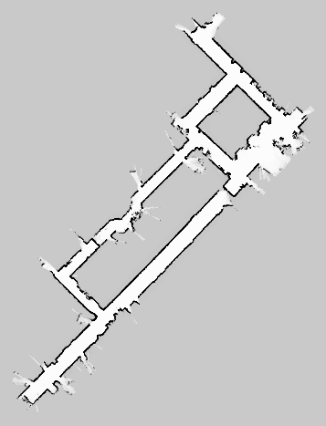
\includegraphics[width=0.23\columnwidth]{./images/volumetric_map_2d.png}
    \end{figure}
    
    \emph{Occupancy Grid Maps} make assumptions about the world.
    
\end{frame}
    
\begin{frame}
    \frametitle{Occupancy Grid Map Assumptions}
    \note{Information taken from https://youtu.be/v-Rm9TUG9LA}
    
    \begin{block}{Assumption 1}
    The area of a cell is either completely free or occupied.
    \end{block}
    
    This assumption does not hold in reality, as there may be objects that are smaller than the cell size or objects that partially cover a cell.
    
    \begin{figure}[!h]
        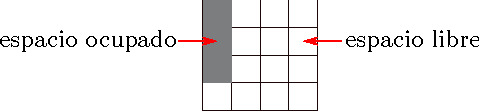
\includegraphics[width=0.7\columnwidth]{./images/grid_map.pdf}
    \end{figure}

\end{frame}
    
\begin{frame}
    \frametitle{Representation: Occupancy Probability}
    \note{information taken from https://youtu.be/v-Rm9TUG9LA}
    
    \begin{itemize}
    \item Each cell is a {\bf binary random variable} that models the cell's occupancy.
    \item The cell is occupied: $p(\map_{i}) = 1$
    \item The cell is free: $p(\map_{i}) = 0$
    \item We have no information: $p(\map_{i}) = 0.5$
    \end{itemize}
    
    \begin{figure}[!h]
    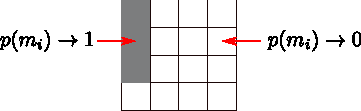
\includegraphics[width=0.7\columnwidth]{./images/grid_map_representation.pdf}
    \end{figure}
    \end{frame}
    
    \begin{frame}
    \frametitle{Occupancy Probability}
    \note{information taken from https://youtu.be/v-Rm9TUG9LA}
    \begin{itemize}
    \item Each cell is a {\bf binary random variable} that models the cell's occupancy.
    \item Notation:
    \begin{itemize}
    \item The probability that the celt is occupied is:\\ $P(\mapRandomVariable_{i} = occ) = P_{occ}(\mapRandomVariable_{i}) = p(\map_{i})$
    \item The probability that the celt is free is:\\ $P(\mapRandomVariable_{i} = free) = P_{free}(\mapRandomVariable_{i}) = 1 - P_{occ}(\mapRandomVariable{i}) = p(\neg \map_{i})$
    \end{itemize}
    \end{itemize}
    
    \end{frame}
    
    \begin{frame}
    \frametitle{Assumption 2}
    \note{information extracted from https://youtu.be/v-Rm9TUG9LA}
    The world is static.
    
    \begin{figure}[!h]
    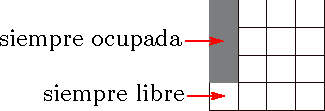
\includegraphics[width=0.7\columnwidth]{./images/grid_map_static_assumption.pdf}
    \end{figure}
    
    This is not true in practice since objects move around the environment or the environment is modified (people walking, objects moving from one place to another, etc.).
    
    \end{frame}
    
    \begin{frame}
    \frametitle{Assumption 3}
    \note{information taken from https://youtu.be/v-Rm9TUG9LA}
    The cells (the random variables) are independent of each other.
    
    \begin{figure}[!h]
    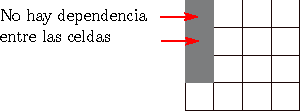
\includegraphics[width=0.7\columnwidth]{./images/grid_map_independency_assumption.pdf}
    \end{figure}
    
    Again, this is not true in practice, but we assume this independence to simplify the model.
    
\end{frame}

\begin{frame}
    \frametitle{Joint Distribution}
    \note{Information taken from https://youtu.be/v-Rm9TUG9LA}
    
    \begin{itemize}
    \item An occupancy map is then the probability distribution representing the entire neighborhood map.
    
    \item The probability distribution of the entire map is the joint probability (\emph{joint belief}) of the values of all individual cells.
    \end{itemize}
    
    \begin{figure}[!h]
    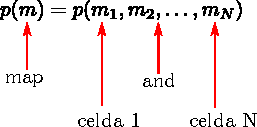
\includegraphics[width=0.5\columnwidth]{./images/joint_distribution.pdf}
    \end{figure}
    
    \end{frame}
    
    \begin{frame}
    \frametitle{Representation}
    \note{Information taken from https://youtu.be/v-Rm9TUG9LA}
    The probability distribution of the map is given by the product of the cells.
    
    \begin{figure}[!h]
    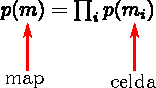
\includegraphics[width=0.3\columnwidth]{./images/map_probability_distribution.pdf}
    \end{figure}
    
    \end{frame}
    
    \begin{frame}
    \frametitle{Estimating a Map from Measurements}
    \note{Information taken from https://youtu.be/v-Rm9TUG9LA}
    
    Given the measurements $\observation_{i:t}$ and the sensor poses $\state_{1:t}$, we estimate the map as
    
    \begin{figure}[!h]
    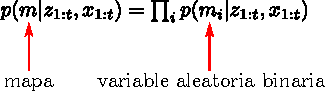
\includegraphics[width=0.5\columnwidth]{./images/map_from_sensor_data.pdf}
    \end{figure}
    
    In this case, we will use range sensors, but we need a sensor that tells us whether a cell is occupied or free.
    
    We can use a {\bf Binary Bayes Filter} to estimate the probability of binary random variables. We assume a static state (map) that does not change over time. An occupied/free cell will always remain occupied/free.
    
\end{frame}

\begin{frame}
	\frametitle{Binary Bayes Filter for Static State}
	\note{información extraída de https://youtu.be/v-Rm9TUG9LA}
    
	\begin{align*}
		\only<1>{
			p(\map_{i}| \observation_{1:t}, \state_{1:t}) \overset{\text{Regla de Bayes}}{=}& \dfrac{p(\observation_{t} | \map_{i}, \observation_{1:t-1}, \state_{1:t}) p(\map_{i} | \observation_{1:t-1}, \state_{1:t})}{p(\observation_{t} | \observation_{1:t-1}, \state_{1:t})}}
		\only<2>{
            p(\map_{i}| \observation_{1:t}, \state_{1:t}) \overset{\text{Regla de Bayes}}{=}& \dfrac{p(\observation_{t} | \map_{i}, \alert{\observation_{1:t-1}}, \alert{\state_{1:t}}) p(\map_{i} | \observation_{1:t-1}, \alert{\state_{1:t}})}{p(\observation_{t} | \observation_{1:t-1}, \state_{1:t})}
		\\
			\overset{\text{Markov}}{=}& \dfrac{p(\observation_{t} | \map_{i}, \state_{t}) p(\map_{i} | \observation_{1:t-1}, \state_{1:t-1})}{p(\observation_{t} | \observation_{1:t-1}, \state_{1:t})}}
		\\
		\only<3>{
            p(\map_{i}| \observation_{1:t}, \state_{1:t}) \overset{\text{Regla de Bayes}}{=}& \dfrac{p(\observation_{t} | \map_{i}, \observation_{1:t-1}, \state_{1:t}) p(\map_{i} | \observation_{1:t-1}, \state_{1:t})}{p(\observation_{t} | \observation_{1:t-1}, \state_{1:t})}
		\\
			\overset{\text{Markov}}{=}& \dfrac{\alert{p(\observation_{t} | \map_{i}, \state_{t})} p(\map_{i} | \observation_{1:t-1}, \state_{1:t-1})}{p(\observation_{t} | \observation_{1:t-1}, \state_{1:t})}
		\\
		    \overset{\text{Regla de Bayes}}{=}& \dfrac{p(\map_{i} | \observation_{t}, \state_{t}) p(\observation_{t} | \state_{t}) p(\map_{i} | \observation_{1:t-1}, \state_{1:t-1})}{p(\map_{i} | \state_{t})p(\observation_{t} | \observation_{1:t-1}, \state_{1:t})}}
		\\
		\only<4>{
            p(\map_{i}| \observation_{1:t}, \state_{1:t}) \overset{\text{Regla de Bayes}}{=}& \dfrac{p(\observation_{t} | \map_{i}, \observation_{1:t-1}, \state_{1:t}) p(\map_{i} | \observation_{1:t-1}, \state_{1:t})}{p(\observation_{t} | \observation_{1:t-1}, \state_{1:t})}
            \\
                \overset{\text{Markov}}{=}& \dfrac{p(\observation_{t} | \map_{i}, \state_{t}) p(\map_{i} | \observation_{1:t-1}, \state_{1:t-1})}{p(\observation_{t} | \observation_{1:t-1}, \state_{1:t})}
            \\
                \overset{\text{Regla de Bayes}}{=}& \dfrac{p(\map_{i} | \observation_{t}, \state_{t}) p(\observation_{t} | \state_{t}) p(\map_{i} | \observation_{1:t-1}, \state_{1:t-1})}{p(\map_{i} | \alert{\state_{t}})p(\observation_{t} | \observation_{1:t-1}, \state_{1:t})}
            \\
		\overset{\text{independencia}}{=}& \dfrac{p(\map_{i} | \observation_{t}, \state_{t}) p(\observation_{t} | \state_{t}) p(\map_{i} | \observation_{1:t-1}, \state_{1:t-1})}{p(\map_{i})p(\observation_{t} | \observation_{1:t-1}, \state_{1:t})}}
	\end{align*}

    \only<2>{We apply Markov:

    The current observation is independent of previous measurements and poses.
    
    Also, in the second term, we can ignore $x_{t}$. That is, knowing my position at time $t$ without having measurements at that time will not help me determine whether a cell is free or occupied. The only case where this can be useful in practice is if the robot is above that cell, and therefore the cell is free of obstacles since it is standing on it.}
    
    \only<3>{We apply Bayes' Rule in the first term of the multiplication}
    
    \only<4>{We assume independence: again, knowing where we are is not useful to know whether a cell is free or occupied.}
    
    \only<5>{Since we are dealing with a binary random variable, we can make the same derivation for the case where the cell is empty
	
	\begin{equation*}
		p(\neg \map_{i}| \observation_{1:t}, \state_{1:t}) \overset{\text{Regla de Bayes}}{=} \dfrac{p(\neg \map_{i} | \observation_{t}, \state_{t}) p(\observation_{t} | \state_{t}) p(\neg \map_{i} | \observation_{1:t-1}, \state_{1:t-1})}{p(\neg \map_{i})p(\observation_{t} | \observation_{1:t-1}, \state_{1:t})}
	\end{equation*}
	}
\end{frame}


\begin{frame}
	\frametitle{Binary Bayes Filter for Static State}
	\note{información extraída de https://youtu.be/v-Rm9TUG9LA}
	
	Let's do a math trick...

    We can compute the ratio of both probabilities by obtaining:
	
    \only<1>{
	\begin{equation*}
		\dfrac{p(\map_{i}| \observation_{1:t}, \state_{1:t})}{p(\neg \map_{i}| \observation_{1:t}, \state_{1:t})} = \dfrac{\dfrac{p(\map_{i} | \observation_{t}, \state_{t}) p(\observation_{t} | \state_{t}) p(\map_{i} | \observation_{1:t-1}, \state_{1:t-1})}{p(\map_{i})p(\observation_{t} | \observation_{1:t-1}, \state_{1:t})}} {\dfrac{p(\neg \map_{i} | \observation_{t}, \state_{t}) p(\observation_{t} | \state_{t}) p(\neg \map_{i} | \observation_{1:t-1}, \state_{1:t-1})}{p(\neg \map_{i})p(\observation_{t} | \observation_{1:t-1}, \state_{1:t})}}
	\end{equation*}
    }

    \only<2>{
	\begin{equation*}
	\dfrac{p(\map_{i}| \observation_{1:t}, \state_{1:t})}{p(\neg \map_{i}| \observation_{1:t}, \state_{1:t})} = \dfrac{\dfrac{p(\map_{i} | \observation_{t}, \state_{t}) \cancel{p(\observation_{t} | \state_{t})} p(\map_{i} | \observation_{1:t-1}, \state_{1:t-1})}{p(\map_{i})\cancel{p(\observation_{t} | \observation_{1:t-1}, \state_{1:t})}}} {\dfrac{p(\neg \map_{i} | \observation_{t}, \state_{t}) \cancel{p(\observation_{t} | \state_{t})} p(\neg \map_{i} | \observation_{1:t-1}, \state_{1:t-1})}{p(\neg \map_{i})\cancel{p(\observation_{t} | \observation_{1:t-1}, \state_{1:t})}}}
	\end{equation*}
    }

    \only<3>{
    \begin{equation*}
        \dfrac{p(\map_{i}| \observation_{1:t}, \state_{1:t})}{p(\neg \map_{i}| \observation_{1:t}, \state_{1:t})} = \dfrac{\dfrac{p(\map_{i} | \observation_{t}, \state_{t}) p(\map_{i} | \observation_{1:t-1}, \state_{1:t-1})}{p(\map_{i})}} {\dfrac{p(\neg \map_{i} | \observation_{t}, \state_{t}) p(\neg \map_{i} | \observation_{1:t-1}, \state_{1:t-1})}{p(\neg \map_{i})}}
    \end{equation*}
    }

    \only<4->{
    \begin{align*}
        \dfrac{p(\map_{i}| \observation_{1:t}, \state_{1:t})}{p(\neg \map_{i}| \observation_{1:t}, \state_{1:t})} 
        =& \dfrac{p(\map_{i} | \observation_{t}, \state_{t}) p(\map_{i} | \observation_{1:t-1}, \state_{1:t-1}) p(\neg \map_{i})} {p(\neg \map_{i} | \observation_{t}, \state_{t}) p(\neg \map_{i} | \observation_{1:t-1}, \state_{1:t-1})p(\map_{i})}\\
    \only<5>{
        =& \dfrac{p(\map_{i} | \observation_{t}, \state_{t})}{1 - p(\map_{i} | \observation_{t}, \state_{t})}
        %
        \dfrac{p(\map_{i} | \observation_{1:t-1}, \state_{1:t-1})}{1- p(\map_{i} | \observation_{1:t-1}, \state_{1:t-1})}
        %
        \dfrac{1 - p(\map_{i})} {p(\map_{i})}
    }
    \only<6>{
        =& \underbrace{\dfrac{p(\map_{i} | \observation_{t}, \state_{t})}{1 - p(\map_{i} | \observation_{t}, \state_{t})}}_{\text{usa } \observation_{t}}
        %
        \underbrace{\dfrac{p(\map_{i} | \observation_{1:t-1}, \state_{1:t-1})}{1- p(\map_{i} | \observation_{1:t-1}, \state_{1:t-1})}}_{\text{término recursivo}}
        %
        \underbrace{\dfrac{1 - p(\map_{i})} {p(\map_{i})}}_{\text{prior}}
    }
    \end{align*}
    }

    \only<5>{Rewrite and Regroup Terms}
    \only<6>{
    \begin{itemize}
        \item The first term uses current information.
        \item The second term uses information from the past.
        \item The third term is a prior (information we assume from the map)
    \end{itemize}
    }
\end{frame}


\begin{frame}
    \frametitle{From Ratio to Probability}
    \note{Information taken from https://youtu.be/v-Rm9TUG9LA}
    
    We can easily transform this ratio, called \emph{odds ratio}, into a probability:
    
    \begin{align*}
    Odds(x) &= \dfrac{p(x)}{1-p(x)}\\
    p(x) &= Odds(x) - Odds(x) p(x)\\
    p(x)(1 + Odds(x)) &= Odds(x)\\
    p(x) &= \dfrac{Odds(x)}{1 + Odds(x)}\\
    p(x) &= \dfrac{1}{1 + \dfrac{1}{Odds(x)}}
    \end{align*}
    
    In this way, we can convert odds to probabilities and from probabilities to odds.
    
    \end{frame}
    
    
    \begin{frame}
     \frametitle{From ratio to probability}
     \note{information taken from https://youtu.be/v-Rm9TUG9LA}
    
     Using $p(x) = \dfrac{1}{1 + \dfrac{1}{Odds(x)}}$ in the odds ratio that we had found
    
     \begin{equation*}
     \dfrac{p(\map _{i}| \observation _{1:t}, \state _{1:t})}{p(\neg \map _{i}| \observation _{1:t}, \state _{1:t})} = \dfrac{p(\map _{i} | \observation _{t}, \state _{t})}{1 - p(\map _{i} | \observation _{t}, \state _{t})}
     %
     \dfrac{p(\map _{i} | \observation _{1:t-1}, \state _{1:t-1})}{1- p(\map _{i} | \observation _{1:t-1}, \state _{1:t-1})}
     %
     \dfrac{1 - p(\map_{i})} {p(\map_{i})}
     \end{equation*}
    
    we then have:
    
     \begin{equation*}
     p(\map_{i}| \observation _{1:t}, \state _{1:t}) =
     \left[
     1 +
     \dfrac{1 - p(\map _{i} | \observation _{t}, \state _{t})}{p(\map _{i} | \observation _{t}, \state _{t})}
     %
     \dfrac{1- p(\map_{i} | \observation_{1:t-1}, \state_{1:t-1})}{p(\map_{i} | \observation_{1:t-1}, \state_{1:t-1})}
    %
    \dfrac{p(\map_{i})}{1 - p(\map_{i})}
    \right]^{-1}
    \end{equation*}
    
    For efficiency reasons, calculations are performed by applying the logarithm to the odds ratio (\emph{log odds} notation).
\end{frame}

\begin{frame}
    \frametitle{log-odds notation}
    \note{information taken from https://youtu.be/v-Rm9TUG9LA}
    \begin{equation*}
    \dfrac{p(\map _{i}| \observation _{1:t}, \state _{1:t})}{1 - p(\map _{i}| \observation _{1:t}, \state _{1:t})} = \underbrace{\dfrac{p(\map _{i} | \observation _{t}, \state _{t})}{1 - p(\map _{i} | \observation _{t}, \state_{t})}}_{\text{use } \observation_{t}}
    %
    \underbrace{\dfrac{p(\map_{i} | \observation_{1:t-1}, \state _{1:t-1})}{1- p(\map _{i} | \observation _{1:t-1}, \state _{1:t-1})}}_{\text{recursive term}}
    %
    \underbrace{\dfrac{1 - p(\map _{i})} {p(\map _{i})}}_{\text{prior}}
    \end{equation*}
   
    \begin{equation*}
    I
    \end{equation*}
   
    Applying A logarithm on both sides, then, on the right side of the equality, multiplications are converted into additions, making the algorithm fast since we only have to apply three additions.
   
   \end{frame}
   
   \begin{frame}
    \frametitle{log-odds notation}
    \note{information taken from https://youtu.be/v-Rm9TUG9LA}
   
    \begin{itemize}
    \item Log odds ratio is defined by:
    \begin{equation*}
    l(x) = \log \dfrac{p(x)}{1-p(x)}
    \end{equation*}
    \item we can solve for $p(x)$
    \begin{equation*}
    p(x) = 1 - \dfrac{1}{1 + \exp l(x)}
    \end{equation*}
    \end{itemize}
   
   \end{frame}
   
   \begin{frame}
    \frametitle{Occupancy mapping using Log Odds}
    \note{information taken from https://youtu.be/v-Rm9TUG9LA}
   
    \begin{itemize}
    \item Log odds ratio is defined by:
    \begin{equation*}
    l(\map _{i}| \observation _{1:t}, \state _{1:t}) = \underbrace{l(\map _{i}| \observation _{t}, \state _{t})}_{\text{inverse sensor model}} + \underbrace{l(\map _{i}| \observation _{1:t-1}, \state _{1:t-1})}_{\text{recursive term}} - \underbrace{l(\map_{i})}_{\text{prior}}
    \end{equation*}
    \item rewriting:
    \begin{equation*}
    l_{t,i} = inv\_sensor\_model(\map_{i}, \state_{t}, \observation_{t}) + l_{t-1,i} - l_{0}
   \end{equation*}
   \end{itemize}
   
   Then, the value of cell $i$ at time $t$ is updated by the sum of the $inv\_sensor\_model$ (a term that depends on my current observation) and the previous value of cell $i$, minus the information prior.
   
\end{frame}

\begin{frame}
    \frametitle{Forward measurement model vs. inverse measurement model}
    \note{information taken from https://youtu.be/v-Rm9TUG9LA}
    
    \TODO{better explain inverse sensor model and forward sensor model}
    
    The \emph{occupancy grid mapping} algorithm requires a marginalized inverse measurement model, $p(\map_{i}|\state, \observation )$. This probability is called inverse because it reasons from effects to causes: it provides information about the world conditioned on a measurement caused by that world.
    
    \emph{inverse models} are often used in situations where the measurements are more complex than the binary state. An example of such a situation is the problem of estimating whether a door is closed or not from camera images. Here, the state is extremely simple, but the space of all the measurements is enormous. It is therefore easier to design a function that calculates the probability of a door being closed from an image than to describe the probability distribution over all images showing a closed door. In other words, it is easier to implement an inverse sensor model than a forward one.
    
    Forward measurement model vs. inverse measurement model
    \url{https://www.cs.cmu.edu/~thrun/papers/thrun.occ-journal.pdf}
    \url{http://robots.stanford.edu/papers/thrun.iros01-occmap.pdf}
    
    Forward models describe the physics of the environment, from causes (occupancy) to effects (measurements). They are denoted $p(\observation | \map)$.
    
    \end{frame}
    
    \begin{frame}
    \frametitle{Occupancy Mapping Algorithm}
    \note{information taken from https://youtu.be/v-Rm9TUG9LA}
    
    \begin{algorithmic}[1]
    \State occupancy\_grid\_mapping($\left\lbrace l_{t-1,i} \right\rbrace, \state_{t}, \observation_{t}$)
    \For {all cells $\map_{i}$}
    \If{$\map_{i}$ is being observed by $\observation_{t}$}
    \State $l_{t,i} = inv\_sensor\_model(\map_{i}, \state_{t}, \observation_{t}) + l_{t-1,i} - l_{0}$
    \Else
    \State $l_{t,i} = l_{t-1,i}$
    \EndIf
    \EndFor
    
    \State \Return $\left\lbrace l_{t,i} \right\rbrace$
    \end{algorithmic}
    Very efficient, since we only have to do sums!
    \note{Moravec and Elfes proposed occupancy grid mapping in the 1980s. Developed for noisy sonar sensors. Also called Mapping with Known Poses}
    
    \end{frame}
    
    \begin{frame}
    \frametitle{Inverse Sensor Model for Laser Range Finder}
    \note{Information taken from https://youtu.be/v-Rm9TUG9LA}
    
    \begin{figure}[!h]
    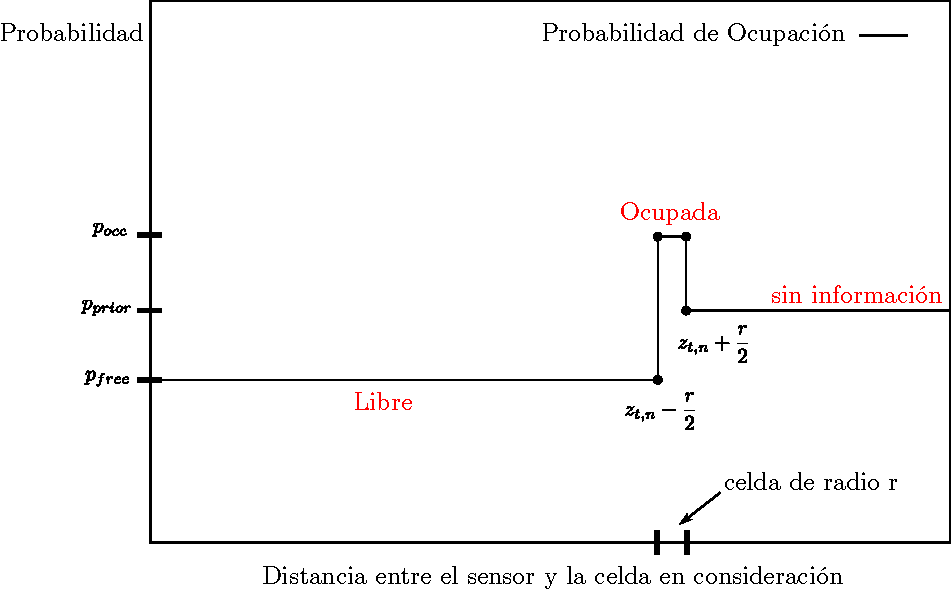
\includegraphics[width=0.8\columnwidth]{./images/inverse_senor_model_range_finder.pdf}
    \end{figure}
    
    \end{frame}
    
    \begin{frame}
    \frametitle{Which cells to update for each LiDAR ray}
    \note{Information taken from https://youtu.be/v-Rm9TUG9LA}
    Bresenham's Line Algorithm
    \begin{figure}[!h]
    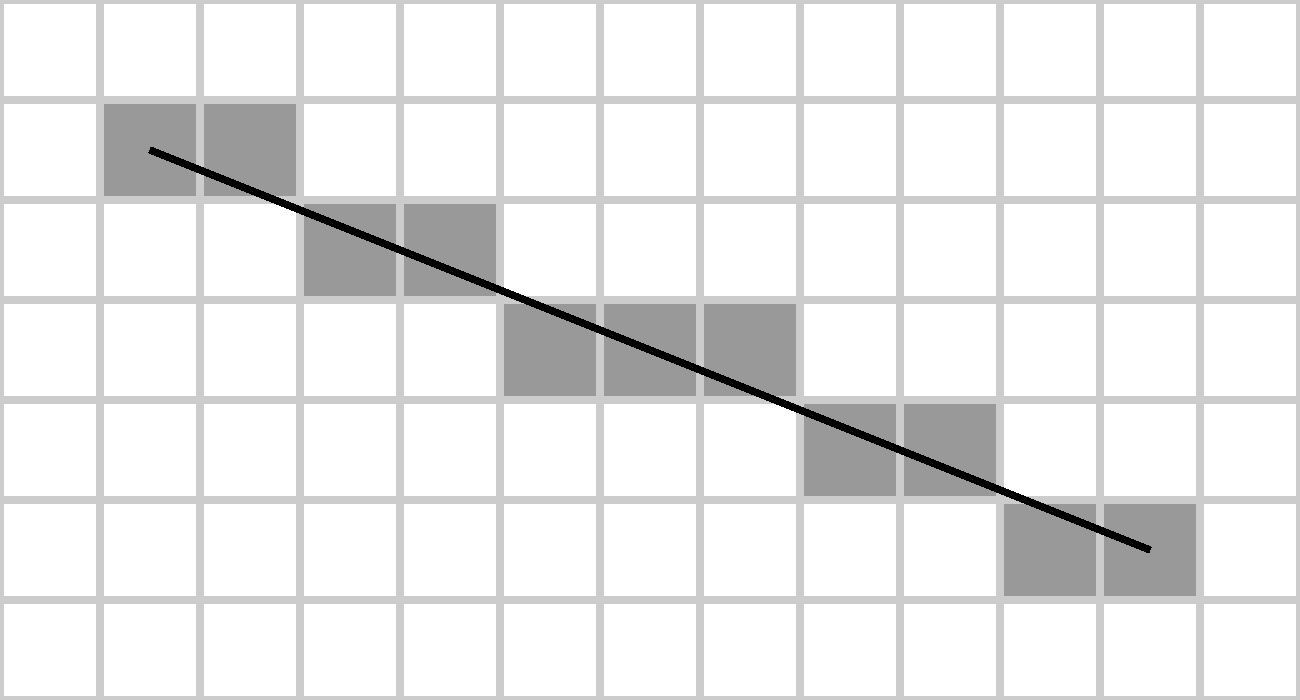
\includegraphics[width=0.6\columnwidth]{./images/bresenham.pdf}
    \end{figure}
    
    Bresenham's line algorithm allows you to draw A line that determines which grid cells should be selected to approximate a straight line between two points.
    
    \end{frame}
    
    \begin{frame}
    \frametitle{From Laser Scans to Occupancy Grid Maps}
    \note{Information taken from https://youtu.be/v-Rm9TUG9LA}
    
    \begin{figure}[!h]
    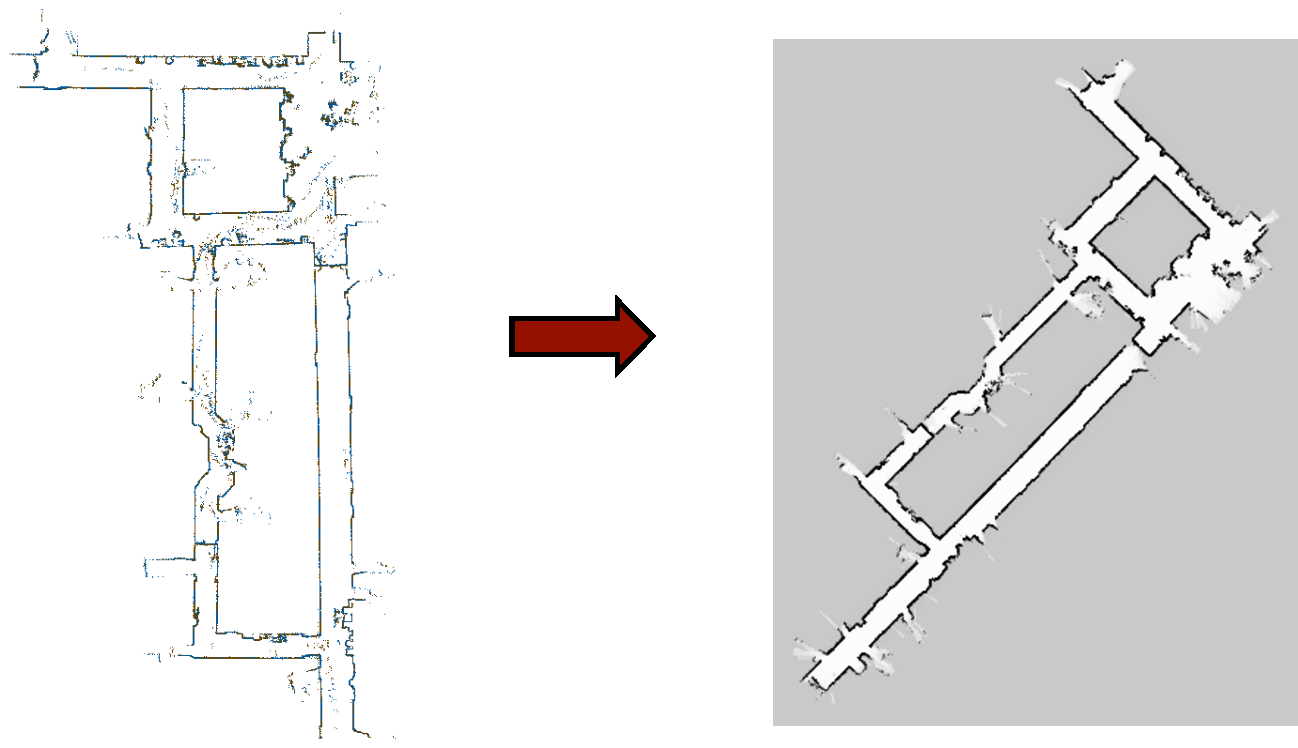
\includegraphics[width=0.6\columnwidth]{./images/laser_scans_to_maps.pdf}
    \end{figure}
    
    \end{frame}
    
\begin{frame}
    \frametitle{Example: Occupancy Grid Map}
    \note{información extraída de https://youtu.be/v-Rm9TUG9LA}
    
    \note{Video tomado de https://www.youtube.com/watch?v=ykOTfrS5pO4}

    \begin{center}
        \movie[autostart,loop,poster]{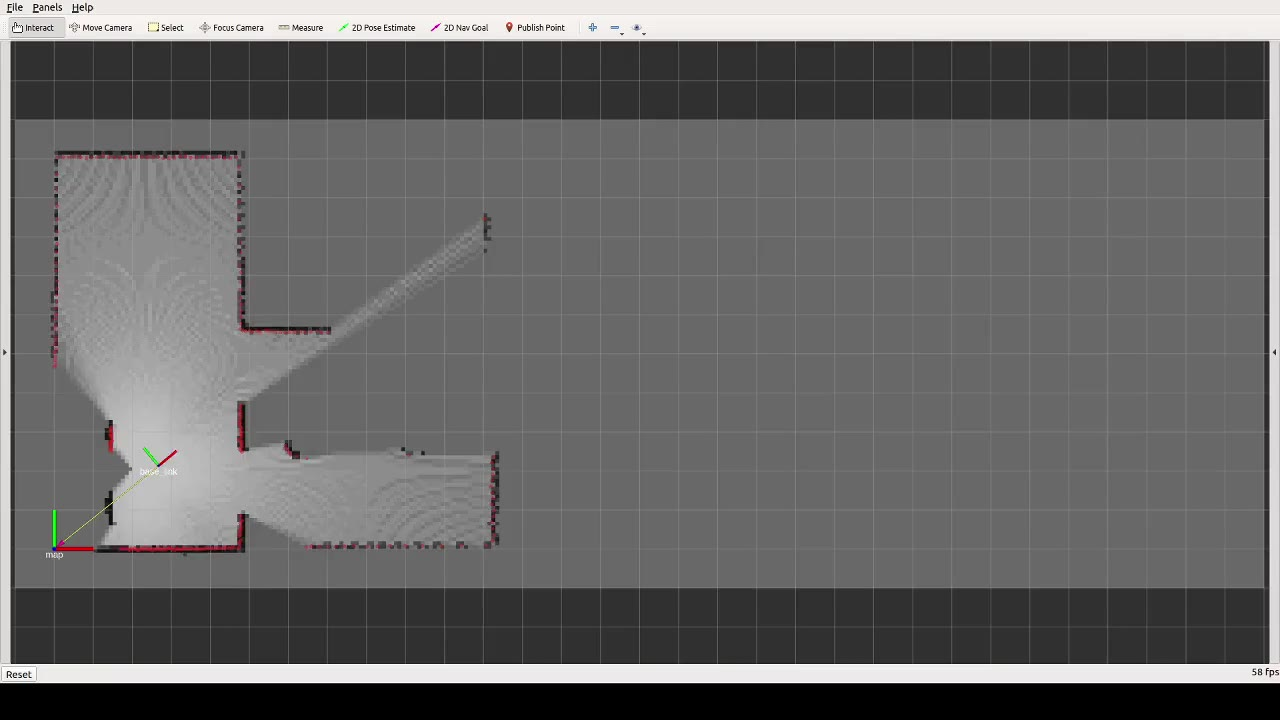
\includegraphics[width=0.8\columnwidth]{./images/occupancy_grid_map_video.jpg}}{./videos/occupancy_grid_map.mp4}
    \end{center}
        
\end{frame}
\begin{frame}
    \frametitle{Summary: Occupancy Grid Map}
    \note{Information taken from https://youtu.be/v-Rm9TUG9LA}
    \begin{itemize}
    \item Occupancy grid maps discretize space into independent cells.
    \item Each cell is a binary random variable that estimates whether the cell is occupied.
    \item Static-state binary Bayes filter per cell.
    \item Mapping with known poses is easy.
    \item The log odds model is fast to compute.
    \item No predefined features are needed.
    \end{itemize}
    
    \end{frame}
    
    \begin{frame}
    \frametitle{Material for assembling these slides}
    
    \begin{itemize}
    \item Course by Cyrill Stachniss: \url{https://youtu.be/v-Rm9TUG9LA}
    
    \item Course by Cyrill Stachniss (slides): \url{http://ais.informatik.uni-freiburg.de/teaching/ws12/mapping/pdf/slam11-gridmaps-4.pdf}
     \end{itemize}
\end{frame}

	\section{Bibliography}
	\begin{frame}
	\frametitle{Bibliography}
   
    Static state binary Bayes filter:
    
    Capítulo 4.2 de \cite{thrun2005probabilistic}
    
    Occupancy Grid Mapping:
    
    Capítulo 9.1 y 9.2 de \cite{thrun2005probabilistic}
	
	\printbibliography
	
\end{frame}

\end{document}